\documentclass{acm}

\usepackage{fontawesome}
\usepackage{etoolbox}
\usepackage{textcomp}
\usepackage[nodisplayskipstretch]{setspace}
\usepackage{xspace}
\usepackage{verbatim}
\usepackage{multicol}
\usepackage{soul}
\usepackage{attrib}

\usepackage{amsmath,amssymb,amsthm}

\usepackage[linesnumbered,commentsnumbered,ruled,vlined]{algorithm2e}
\newcommand\mycommfont[1]{\footnotesize\ttfamily\textcolor{blue}{#1}}
\SetCommentSty{mycommfont}
\SetKwComment{tcc}{ \# }{}
\SetKwComment{tcp}{ \# }{}

\usepackage{siunitx}

\usepackage{tikz}
\usepackage{pgfplots}
\usetikzlibrary{decorations.pathreplacing,calc,arrows.meta,shapes,graphs}

\AtBeginEnvironment{minted}{\singlespacing\fontsize{10}{10}\selectfont}
\setmainfont{Open Sans Light}
\usefonttheme{serif}

\makeatletter
\patchcmd{\beamer@sectionintoc}{\vskip1.5em}{\vskip0.5em}{}{}
\makeatother

% Math stuffs
\newcommand{\Z}{\mathbb{Z}}
\newcommand{\R}{\mathbb{R}}
\newcommand{\N}{\mathbb{N}}
\newcommand{\lcm}{\text{lcm}}
\newcommand{\Inn}{\text{Inn}}
\newcommand{\Aut}{\text{Aut}}
\newcommand{\Ker}{\text{Ker}\ }
\newcommand{\la}{\langle}
\newcommand{\ra}{\rangle}

\newcommand{\yournewcommand}[2]{Something #1, and #2}

\newenvironment{question}[1]{\par\textbf{Question #1.}\par}{}

\newcommand{\pmidg}[1]{\parbox{\widthof{#1}}{#1}}
\newcommand{\splitslide}[4]{
    \noindent
    \begin{minipage}{#1 \textwidth - #2 }
        #3
    \end{minipage}%
    \hspace{ \dimexpr #2 * 2 \relax }%
    \begin{minipage}{\textwidth - #1 \textwidth - #2 }
        #4
    \end{minipage}
}

\newcommand{\frameoutput}[1]{\frame{\colorbox{white}{#1}}}

\newcommand{\tikzmark}[1]{%
\tikz[baseline=-0.55ex,overlay,remember picture] \node[inner sep=0pt,] (#1)
{\vphantom{T}};
}

\newcommand{\braced}[3]{%
    \begin{tikzpicture}[overlay,remember picture]
        \draw [thick,decorate,decoration={brace,raise=1ex,amplitude=4pt},blue] (#2.south west-|T1.south west) -- node[anchor=west,left,xshift=-1.8ex,text=olive]{#3} (#1.north west-|T1.south west);
    \end{tikzpicture}
}

\title{Matrix: An open network for secure, decentralized communication}
\author{Sumner Evans}
\date{August 31, 2021}
\institute{Beeper}

\begin{document}

\begin{frame}{A bit about me}
    \begin{itemize}
        \item I graduated in 2018 with my bachelor's in CS from Mines.
        \item I graduated in 2019 with my master's in CS, also from Mines.
        \item I worked at The Trade Desk for two years right after graduating.
        \item I currently am teaching \textit{CSCI 400 Principles of Programming
            Languages} and I have previously taught \textit{CSCI 406 Algorithms}
            and \textit{CSCI 564 Advanced Computer Architecture}.
        \item I started at Beeper in July.
    \end{itemize}
\end{frame}

\begin{frame}{A bit about you}
    I'd like to get to know everyone a bit more and get a feel for everyone's
    experience levels.
    \pause

    \begin{itemize}[<+->]
        \item How many of you have taken Algorithms?
        \item How many of you have taken Data Structures?
        \item How many of you have taken Intro to Computer Science?
        \item How many of you are in the ACM Matrix chat?
    \end{itemize}
    \pause[\thebeamerpauses]

    I know you have all had a year of Zoom-class where asking questions is hard,
    but now there are no excuses: interrupt me at any time if I use a term you
    don't understand.
\end{frame}

\begin{frame}{Overview}
    \setbeamertemplate{section in toc}[sections numbered]
    \tableofcontents[hideallsubsections]
\end{frame}

\section{Why Matrix?}

\begin{frame}{Let's talk about chat platforms\ldots}
    Which of the following chat networks do you use/have you used?
    \begin{multicols}{2}
        \begin{itemize}[<+->]
            \item SMS/MMS
            \item iMessage
            \item LinkedIn
            \item Snapchat
            \item WhatsApp
            \item Instagram
            \item Discord
            \item Facebook Messenger
            \item Hangouts
            \item Slack
            \item Microsoft Teams
            \item Signal
            \item Telegram
            \item Wire
        \end{itemize}
    \end{multicols}
    \pause[\thebeamerpauses]
    What do all of these chat networks have in common?
    \pause

    They are \textbf{non-interoperable, and many are closed source and/or
    unencrypted}.
\end{frame}

\begin{frame}{Why is this a problem?}
    The \textbf{closed source} platforms are problematic because you can never
    be sure \textit{how your data is being used}.
    \pause

    The \textbf{unencrypted} platforms are problematic because your messages are
    not private.
    \pause

    And, because none of them are interoperable, you have to have a ton of chat
    apps on your phone.
\end{frame}

\section{What does Matrix provide?}

\begin{frame}{Matrix solves all your problems}
    Matrix is an \textbf{open} specification for \textbf{encrypted},
    \textbf{decentralized} communication. \pause

    It is also designed in such a way that it makes it easy to break down walled
    garden communication platforms via \textbf{bridging}.

    % TODO diagram of bridging
\end{frame}

\begin{frame}{A side note}
    I first became interested in Matrix when I was the incoming Chair of ACM.
    Robby (VC) and I tried out most of the open source chat platforms and ended
    up landing on Matrix because it had all of these characteristics.
\end{frame}

\begin{frame}{Matrix is an \textit{open specification}}
    Open specifications and standards are all around you. They just make
    sense\texttrademark.

    Examples:\pause
    \begin{itemize}
        \item Power plugs
        \item USB
        \item Wi-Fi
        \item Every crypto algorithm that's any good
    \end{itemize}
    \pause

    Open protocols allow for \textit{open development} and  \textit{clean-room
    implementations}, they \textit{encourage competition}, and are
    \textit{externally auditable}.
\end{frame}

\begin{frame}{Matrix is \textit{encrypted} by default*}
    Matrix has encryption built-in. It is implemented using Olm, which is a
    clone of the Signal protocol

    % TODO add more here
\end{frame}

\begin{frame}{Matrix is \textit{decentralized}}
    The Matrix architecture is actually a \textit{federated} architecture.

    Individual devices communicate to a \textit{homeserver} which anyone can
    host.

    The homeserver communicates with other homeservers in the federation.
    \pause

    Think of it like email. You can email somebody using Outlook from Gmail.*
    \pause

    Every server in the federation gets a copy of a room, so no one entity
    controls the network.
    \pause

    This also means that the network is resilient to individual server outages,
    or even wider internet outages.
\end{frame}

\begin{frame}{Matrix allows for \textit{bridges} and \textit{bots}}
    Bridges bring external chat networks into Matrix. More on this later.
    \pause

    Bots allow for automated interactions and notifications.
\end{frame}

\section{How does it work?}

\begin{frame}{Architecture}
    Every server has a copy of the room, but how do we keep that in sync?
    \pause

    The architecture of Matrix does this in a way that ensures \textit{eventual
    consistency}.
    \pause

    Even if the server where the room was created goes down, people can still
    communicate.

    When a broken server comes back online, it will receive all the
    \textit{events} (messages).
    \pause

    Let's look at the animation on Matrix.org\ldots
\end{frame}

\begin{frame}[fragile]{Client-Server API}
    The \textbf{Client-Server API} specifies how clients communicate with their
    homeserver.
    \pause
    \vspace{1in}

    \Huge
    \textbf{Demo!}
\end{frame}

\begin{frame}{Federation (Server-Server) API}
    The \textbf{Server-Server API} or \textbf{Federation API} specifies how
    servers communicate with other servers to ensure that everyone has the same
    room state.
\end{frame}

\begin{frame}{A bit of graph theory}
    \begin{columns}
    \begin{column}{0.6\textwidth}
        \begin{itemize}[<+->]
            \item A \textbf{graph} is a collection of \textit{nodes} connected by
                \textit{edges}.
            \item A \textbf{directed graph} is a graph where the edges are
                \textit{directional} (have arrows).
            \item An \textbf{acyclic graph} is a graph that has no cycles/loops.
            \item A \textbf{directed acyclic graph (DAG)} is a directional graph
                with no cycles.
        \end{itemize}
    \end{column}%%
    \begin{column}{0.4\textwidth} %%
        \only<4>{
            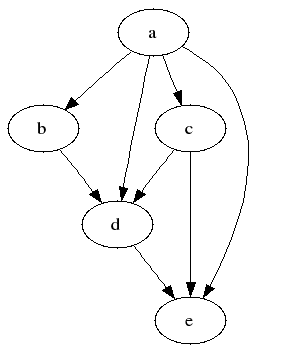
\includegraphics[width=\textwidth]{graphics/dag}
        }
    \end{column}
    \end{columns}
\end{frame}

\begin{frame}{The event DAG}
    Matrix rooms are represented by a DAG of \textit{events} representing things
    such as messages, joins, leaves, etc.
    \pause

    The DAG provides a \textit{partial ordering} of events in the room because
    every event has zero or more ``parent'' events.
    \pause

    This is similar to Git where every commit has 0 or more ``parent'' commits.

    \vspace{1cm}
    {
        \tiny
        See \url{https://matrix.org/docs/spec/\#event-graphs}
    }
\end{frame}

\begin{frame}{Event types}
    There are two main event types: \textbf{message events} and \textbf{state
    events}.
    \pause

    \textbf{Message events:} \\
    These describe transient `once-off' activity in a room such as an instant
    messages, VoIP call setups, file transfers, etc. They generally describe
    communication activity.
    \pause

    \textbf{State events:} \\
    These describe updates to a given piece of persistent information (`state')
    related to a room, such as the room's name, topic, membership, participating
    servers, etc. State is modelled as a lookup table of key/value pairs per
    room, with each key being a tuple of \texttt{state\_key} and \texttt{event
    type}. Each state event updates the value of a given key.

    {
        \tiny
        See \url{https://matrix.org/docs/spec/\#room-structure}
    }
\end{frame}

\section{What does Beeper do?}

% bridges
% clients which are forks of element

\section{Things that I'm excited about in Matrix}

\begin{frame}
  * Obviously excited about bridges
  * Excited about possibilities with bots
  * Excited about possibilities of building on top of Matrix. For example,
    matrix notepad and matrix board
  * Excited about spaces and the potential for better community management
\end{frame}

\section{How to get involved with Matrix}

\section{A few general tips for everyone}

\end{document}
% Local Variables:
% TeX-command-extra-options: "-shell-escape"
% End:
